\section{moeo\-Elitist\-Replacement$<$ EOT, Worth\-T $>$ Class Template Reference}
\label{classmoeoElitistReplacement}\index{moeoElitistReplacement@{moeoElitistReplacement}}
Keep all the best individuals (almost cut-and-pasted from {\bf eo\-NDPlus\-Replacement}, (c) Maarten Keijzer, Marc Schoenauer and Ge\-Neura Team, 2002).  


{\tt \#include $<$moeo\-Replacement.h$>$}

Inheritance diagram for moeo\-Elitist\-Replacement$<$ EOT, Worth\-T $>$::\begin{figure}[H]
\begin{center}
\leavevmode
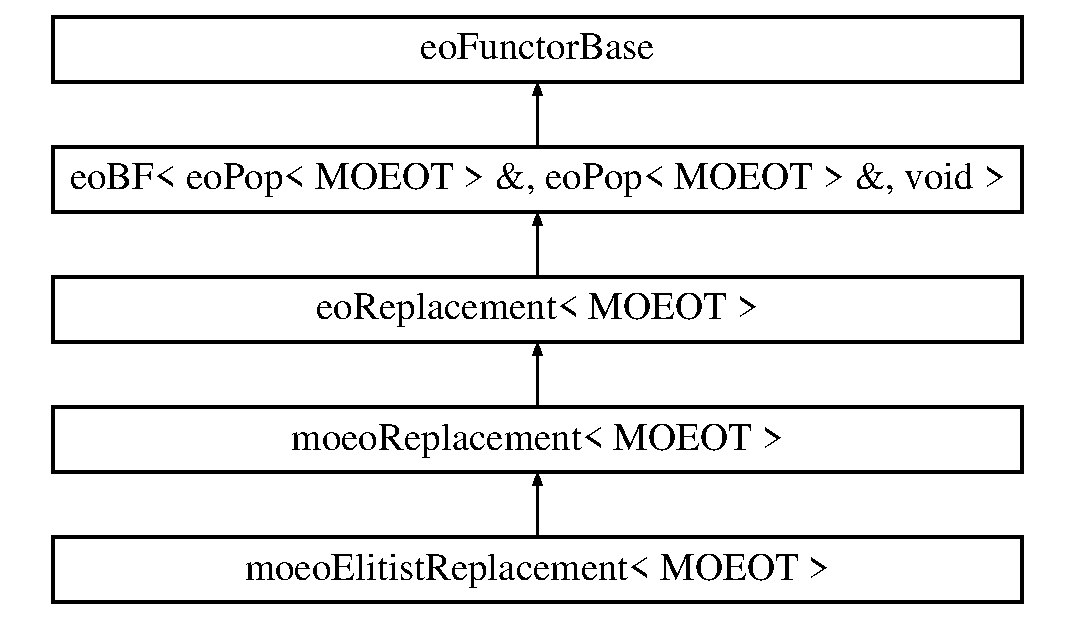
\includegraphics[height=5cm]{classmoeoElitistReplacement}
\end{center}
\end{figure}
\subsection*{Public Member Functions}
\begin{CompactItemize}
\item 
{\bf moeo\-Elitist\-Replacement} ({\bf eo\-Perf2Worth}$<$ EOT, Worth\-T $>$ \&\_\-perf2worth)
\begin{CompactList}\small\item\em constructor \item\end{CompactList}\item 
void {\bf operator()} ({\bf eo\-Pop}$<$ EOT $>$ \&\_\-parents, {\bf eo\-Pop}$<$ EOT $>$ \&\_\-offspring)
\begin{CompactList}\small\item\em replacement - result in \_\-parents \item\end{CompactList}\end{CompactItemize}
\subsection*{Private Attributes}
\begin{CompactItemize}
\item 
{\bf eo\-Perf2Worth}$<$ EOT, Worth\-T $>$ \& {\bf perf2worth}\label{classmoeoElitistReplacement_020f0e0b6b88a0081d922cca5b05990e}

\begin{CompactList}\small\item\em the functor object to transform raw fitnesses into fitness for selection \item\end{CompactList}\end{CompactItemize}


\subsection{Detailed Description}
\subsubsection*{template$<$class EOT, class Worth\-T = double$>$ class moeo\-Elitist\-Replacement$<$ EOT, Worth\-T $>$}

Keep all the best individuals (almost cut-and-pasted from {\bf eo\-NDPlus\-Replacement}, (c) Maarten Keijzer, Marc Schoenauer and Ge\-Neura Team, 2002). 



Definition at line 35 of file moeo\-Replacement.h.

\subsection{Constructor \& Destructor Documentation}
\index{moeoElitistReplacement@{moeo\-Elitist\-Replacement}!moeoElitistReplacement@{moeoElitistReplacement}}
\index{moeoElitistReplacement@{moeoElitistReplacement}!moeoElitistReplacement@{moeo\-Elitist\-Replacement}}
\subsubsection{\setlength{\rightskip}{0pt plus 5cm}template$<$class EOT, class Worth\-T = double$>$ {\bf moeo\-Elitist\-Replacement}$<$ EOT, Worth\-T $>$::{\bf moeo\-Elitist\-Replacement} ({\bf eo\-Perf2Worth}$<$ EOT, Worth\-T $>$ \& {\em \_\-perf2worth})\hspace{0.3cm}{\tt  [inline]}}\label{classmoeoElitistReplacement_fa62ed508ac194ed7b720e37dd22458c}


constructor 

\begin{Desc}
\item[Parameters:]
\begin{description}
\item[{\em \_\-perf2worth}]the functor class to transform raw fitnesses into fitness for selection \end{description}
\end{Desc}


Definition at line 43 of file moeo\-Replacement.h.

\subsection{Member Function Documentation}
\index{moeoElitistReplacement@{moeo\-Elitist\-Replacement}!operator()@{operator()}}
\index{operator()@{operator()}!moeoElitistReplacement@{moeo\-Elitist\-Replacement}}
\subsubsection{\setlength{\rightskip}{0pt plus 5cm}template$<$class EOT, class Worth\-T = double$>$ void {\bf moeo\-Elitist\-Replacement}$<$ EOT, Worth\-T $>$::operator() ({\bf eo\-Pop}$<$ EOT $>$ \& {\em \_\-parents}, {\bf eo\-Pop}$<$ EOT $>$ \& {\em \_\-offspring})\hspace{0.3cm}{\tt  [inline, virtual]}}\label{classmoeoElitistReplacement_aad627deb45859e65ace0709c004049a}


replacement - result in \_\-parents 

\begin{Desc}
\item[Parameters:]
\begin{description}
\item[{\em \_\-parents}]parents population \item[{\em \_\-offspring}]offspring population \end{description}
\end{Desc}


Implements {\bf eo\-BF$<$ eo\-Pop$<$ EOT $>$ \&, eo\-Pop$<$ EOT $>$ \&, void $>$}.

Definition at line 54 of file moeo\-Replacement.h.

The documentation for this class was generated from the following file:\begin{CompactItemize}
\item 
moeo\-Replacement.h\end{CompactItemize}
